\PassOptionsToPackage{unicode=true}{hyperref} % options for packages loaded elsewhere
\PassOptionsToPackage{hyphens}{url}
%
\documentclass[]{book}
\usepackage{lmodern}
\usepackage{amssymb,amsmath}
\usepackage{ifxetex,ifluatex}
\usepackage{fixltx2e} % provides \textsubscript
\ifnum 0\ifxetex 1\fi\ifluatex 1\fi=0 % if pdftex
  \usepackage[T1]{fontenc}
  \usepackage[utf8]{inputenc}
  \usepackage{textcomp} % provides euro and other symbols
\else % if luatex or xelatex
  \usepackage{unicode-math}
  \defaultfontfeatures{Ligatures=TeX,Scale=MatchLowercase}
\fi
% use upquote if available, for straight quotes in verbatim environments
\IfFileExists{upquote.sty}{\usepackage{upquote}}{}
% use microtype if available
\IfFileExists{microtype.sty}{%
\usepackage[]{microtype}
\UseMicrotypeSet[protrusion]{basicmath} % disable protrusion for tt fonts
}{}
\IfFileExists{parskip.sty}{%
\usepackage{parskip}
}{% else
\setlength{\parindent}{0pt}
\setlength{\parskip}{6pt plus 2pt minus 1pt}
}
\usepackage{hyperref}
\hypersetup{
            pdftitle={Smart Data Project},
            pdfauthor={Hugo Brehier, Florentin Coeurdoux},
            pdfborder={0 0 0},
            breaklinks=true}
\urlstyle{same}  % don't use monospace font for urls
\usepackage{color}
\usepackage{fancyvrb}
\newcommand{\VerbBar}{|}
\newcommand{\VERB}{\Verb[commandchars=\\\{\}]}
\DefineVerbatimEnvironment{Highlighting}{Verbatim}{commandchars=\\\{\}}
% Add ',fontsize=\small' for more characters per line
\usepackage{framed}
\definecolor{shadecolor}{RGB}{248,248,248}
\newenvironment{Shaded}{\begin{snugshade}}{\end{snugshade}}
\newcommand{\AlertTok}[1]{\textcolor[rgb]{0.94,0.16,0.16}{#1}}
\newcommand{\AnnotationTok}[1]{\textcolor[rgb]{0.56,0.35,0.01}{\textbf{\textit{#1}}}}
\newcommand{\AttributeTok}[1]{\textcolor[rgb]{0.77,0.63,0.00}{#1}}
\newcommand{\BaseNTok}[1]{\textcolor[rgb]{0.00,0.00,0.81}{#1}}
\newcommand{\BuiltInTok}[1]{#1}
\newcommand{\CharTok}[1]{\textcolor[rgb]{0.31,0.60,0.02}{#1}}
\newcommand{\CommentTok}[1]{\textcolor[rgb]{0.56,0.35,0.01}{\textit{#1}}}
\newcommand{\CommentVarTok}[1]{\textcolor[rgb]{0.56,0.35,0.01}{\textbf{\textit{#1}}}}
\newcommand{\ConstantTok}[1]{\textcolor[rgb]{0.00,0.00,0.00}{#1}}
\newcommand{\ControlFlowTok}[1]{\textcolor[rgb]{0.13,0.29,0.53}{\textbf{#1}}}
\newcommand{\DataTypeTok}[1]{\textcolor[rgb]{0.13,0.29,0.53}{#1}}
\newcommand{\DecValTok}[1]{\textcolor[rgb]{0.00,0.00,0.81}{#1}}
\newcommand{\DocumentationTok}[1]{\textcolor[rgb]{0.56,0.35,0.01}{\textbf{\textit{#1}}}}
\newcommand{\ErrorTok}[1]{\textcolor[rgb]{0.64,0.00,0.00}{\textbf{#1}}}
\newcommand{\ExtensionTok}[1]{#1}
\newcommand{\FloatTok}[1]{\textcolor[rgb]{0.00,0.00,0.81}{#1}}
\newcommand{\FunctionTok}[1]{\textcolor[rgb]{0.00,0.00,0.00}{#1}}
\newcommand{\ImportTok}[1]{#1}
\newcommand{\InformationTok}[1]{\textcolor[rgb]{0.56,0.35,0.01}{\textbf{\textit{#1}}}}
\newcommand{\KeywordTok}[1]{\textcolor[rgb]{0.13,0.29,0.53}{\textbf{#1}}}
\newcommand{\NormalTok}[1]{#1}
\newcommand{\OperatorTok}[1]{\textcolor[rgb]{0.81,0.36,0.00}{\textbf{#1}}}
\newcommand{\OtherTok}[1]{\textcolor[rgb]{0.56,0.35,0.01}{#1}}
\newcommand{\PreprocessorTok}[1]{\textcolor[rgb]{0.56,0.35,0.01}{\textit{#1}}}
\newcommand{\RegionMarkerTok}[1]{#1}
\newcommand{\SpecialCharTok}[1]{\textcolor[rgb]{0.00,0.00,0.00}{#1}}
\newcommand{\SpecialStringTok}[1]{\textcolor[rgb]{0.31,0.60,0.02}{#1}}
\newcommand{\StringTok}[1]{\textcolor[rgb]{0.31,0.60,0.02}{#1}}
\newcommand{\VariableTok}[1]{\textcolor[rgb]{0.00,0.00,0.00}{#1}}
\newcommand{\VerbatimStringTok}[1]{\textcolor[rgb]{0.31,0.60,0.02}{#1}}
\newcommand{\WarningTok}[1]{\textcolor[rgb]{0.56,0.35,0.01}{\textbf{\textit{#1}}}}
\usepackage{longtable,booktabs}
% Fix footnotes in tables (requires footnote package)
\IfFileExists{footnote.sty}{\usepackage{footnote}\makesavenoteenv{longtable}}{}
\usepackage{graphicx,grffile}
\makeatletter
\def\maxwidth{\ifdim\Gin@nat@width>\linewidth\linewidth\else\Gin@nat@width\fi}
\def\maxheight{\ifdim\Gin@nat@height>\textheight\textheight\else\Gin@nat@height\fi}
\makeatother
% Scale images if necessary, so that they will not overflow the page
% margins by default, and it is still possible to overwrite the defaults
% using explicit options in \includegraphics[width, height, ...]{}
\setkeys{Gin}{width=\maxwidth,height=\maxheight,keepaspectratio}
\setlength{\emergencystretch}{3em}  % prevent overfull lines
\providecommand{\tightlist}{%
  \setlength{\itemsep}{0pt}\setlength{\parskip}{0pt}}
\setcounter{secnumdepth}{5}
% Redefines (sub)paragraphs to behave more like sections
\ifx\paragraph\undefined\else
\let\oldparagraph\paragraph
\renewcommand{\paragraph}[1]{\oldparagraph{#1}\mbox{}}
\fi
\ifx\subparagraph\undefined\else
\let\oldsubparagraph\subparagraph
\renewcommand{\subparagraph}[1]{\oldsubparagraph{#1}\mbox{}}
\fi

% set default figure placement to htbp
\makeatletter
\def\fps@figure{htbp}
\makeatother

\usepackage{booktabs}
\usepackage{amsthm}
\makeatletter
\def\thm@space@setup{%
  \thm@preskip=8pt plus 2pt minus 4pt
  \thm@postskip=\thm@preskip
}
\makeatother
\usepackage[]{natbib}
\bibliographystyle{apalike}

\title{Smart Data Project}
\author{Hugo Brehier, Florentin Coeurdoux}
\date{2020-02-13}

\begin{document}
\maketitle

{
\setcounter{tocdepth}{1}
\tableofcontents
}
\hypertarget{introduction}{%
\chapter{Introduction}\label{introduction}}

\hypertarget{initial-problem}{%
\section{Initial problem}\label{initial-problem}}

Our task involves the training of a classifier specialized in recognizing airplanes constructor and model type.
The idea is to put into practice our courses of Deep Learning, especially Convolution Neural Networks (CNN).
Indeed, these models have gained a lot of traction in the last decade or so, in computer vision, after setting
the best accuracy in classification contests, such as \href{https://mc.ai/paper-review-of-alexnet-caffenet-winner-in-ilsvrc-2012-image-classification/}{\textbf{AlexNet on ImageNet}}.
We will first look into classyfing Airbus and Boeing airplanes. Afterwards, we will delve into model types.
In modern fashion, the data used to train our models is scrapped from the website \href{https://www.planespotters.net/}{\textbf{planespotters.net}}.
To manage the planning and monitoring of the various tasks throughout the project we organized ourselves thanks to a project management website : Trello.

\begin{figure}
\centering
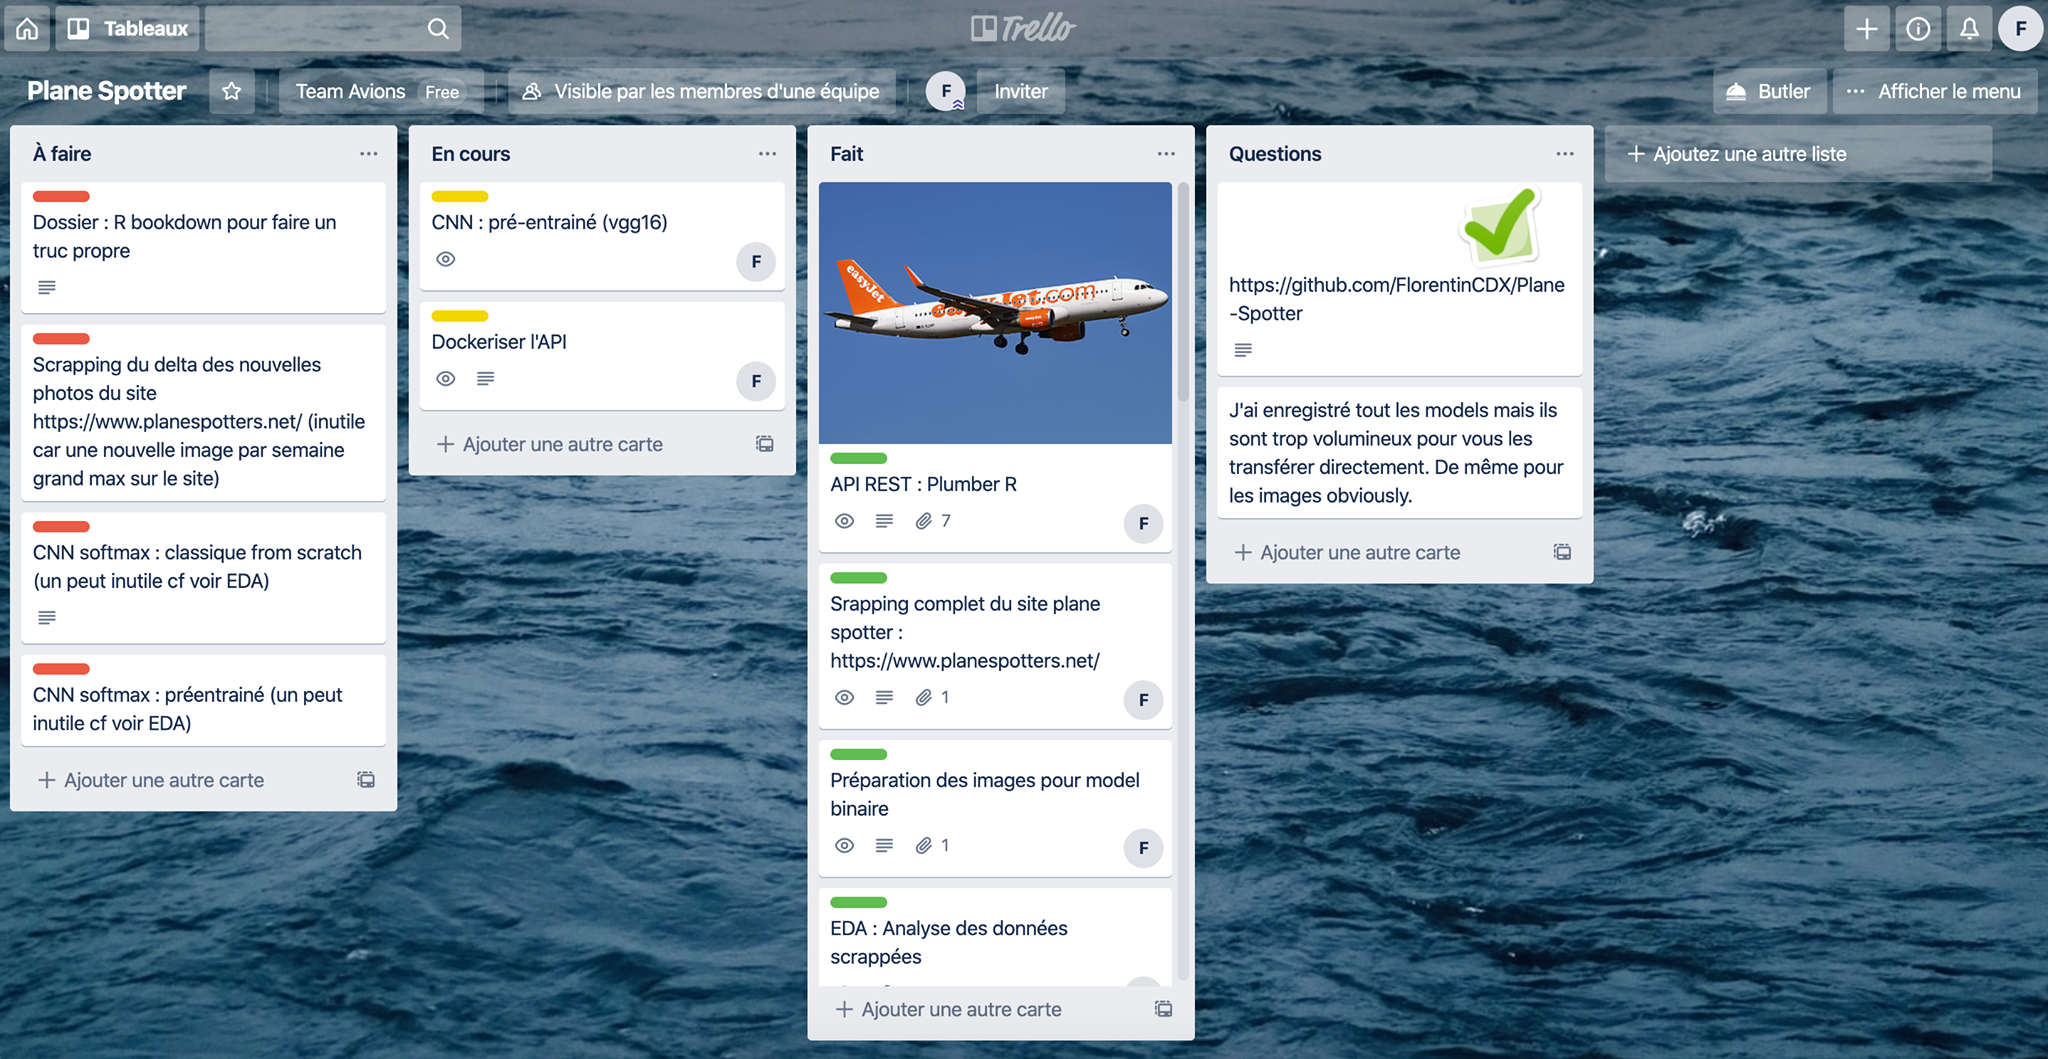
\includegraphics[width=0.75\textwidth,height=\textheight]{trello.png}
\caption{Our trello dashboard}
\end{figure}

\clearpage

\hypertarget{outline}{%
\section{Outline}\label{outline}}

In latter parts, we will describe the following points:

\begin{itemize}
\tightlist
\item
  the available data
\item
  the methods and tools used
\item
  the results obtained
\end{itemize}

The structure of our report will be as follow:

\begin{enumerate}
\def\labelenumi{\arabic{enumi}.}
\tightlist
\item
  Website scrapping
\item
  Exploratory analysis
\item
  Classification through Deep Learning
\item
  Deploying to production
\end{enumerate}

\hypertarget{web-scrapping}{%
\chapter{Web Scrapping}\label{web-scrapping}}

\hypertarget{what-is-web-scraping}{%
\section{What is Web Scraping?}\label{what-is-web-scraping}}

Web scraping is a technique for converting the data present in unstructured format (HTML tags) over the web to the structured format which can easily be accessed and used.

Almost all the main languages provide ways for performing web scraping. To remain consistent in the same programming language we have chosen to use the R language for scraping the data from the planespotters.com website.

\hypertarget{the-available-data}{%
\section{The available data}\label{the-available-data}}

This website contains thousands of aircrafts pictures as well as the information about the constructor, the model and the airline for each different aircraft. Our aim is to extract all these informations.

\hypertarget{website-extraction}{%
\section{Website extraction}\label{website-extraction}}

Fisrt we have to load the different libraries.

\begin{Shaded}
\begin{Highlighting}[]
\KeywordTok{library}\NormalTok{(rvest)}
\KeywordTok{library}\NormalTok{(dplyr)}
\KeywordTok{library}\NormalTok{(stringr)}
\end{Highlighting}
\end{Shaded}

The R package rvest (\citet{R-rvest}) is a package that makes it easy to scrape data from html web pages, inspired by python libraries like beautiful soup. It is designed to work with magrittr so that you can express complex operations as pipelines.

The \textbf{html\_attr} function allows to extract attributes, text and tag name from html.

The website contains 125 pages and each pages contains 48 differents pictures of airplanes with descriptions. Each images

Here is our entire website images extraction :

\begin{Shaded}
\begin{Highlighting}[]
\NormalTok{aicrafts <-}\StringTok{ }\KeywordTok{matrix}\NormalTok{(}\DataTypeTok{ncol =} \DecValTok{3}\NormalTok{, }\DataTypeTok{nrow =} \DecValTok{48}\OperatorTok{*}\DecValTok{125}\NormalTok{)}
\NormalTok{nb <-}\StringTok{ }\DecValTok{0}
\ControlFlowTok{for}\NormalTok{ (i }\ControlFlowTok{in} \DecValTok{1}\OperatorTok{:}\DecValTok{125}\NormalTok{)\{}
\NormalTok{  nb <-}\StringTok{ }\NormalTok{nb}\OperatorTok{+}\DecValTok{1}
\NormalTok{  planespotter_url <-}\StringTok{ }\KeywordTok{paste}\NormalTok{(}\StringTok{"https://www.planespotters.net/photos/latest?page="}\NormalTok{,}
\NormalTok{                            i, }\DataTypeTok{sep =} \StringTok{""}\NormalTok{)}
\NormalTok{  planespotter <-}\StringTok{ }\KeywordTok{read_html}\NormalTok{(planespotter_url)}
\NormalTok{  img <-}\StringTok{ }\NormalTok{planespotter }\OperatorTok
\StringTok{    }\KeywordTok{html_node}\NormalTok{(}\DataTypeTok{xpath =} \StringTok{'//*/img'}\NormalTok{)}
  
\NormalTok{  imgalt <-}\StringTok{ }\KeywordTok{html_attr}\NormalTok{(img, }\StringTok{'alt'}\NormalTok{)}
\NormalTok{  imgsrc <-}\StringTok{ }\KeywordTok{html_attr}\NormalTok{(img, }\StringTok{'src'}\NormalTok{)}
\NormalTok{  imgsrc_split <-}\StringTok{ }\KeywordTok{strsplit}\NormalTok{(imgsrc, }\StringTok{"_"}\NormalTok{)}
\NormalTok{  img_number <-}\StringTok{ }\KeywordTok{as.integer}\NormalTok{(imgsrc_split[[}\DecValTok{1}\NormalTok{]][}\DecValTok{3}\NormalTok{])}
  
\NormalTok{  constructor_html <-}\StringTok{ }\NormalTok{planespotter }\OperatorTok
\StringTok{    }\KeywordTok{html_nodes}\NormalTok{(}\KeywordTok{paste0}\NormalTok{(}\StringTok{'#'}\NormalTok{, img_number, }\StringTok{" a"}\NormalTok{)) }\OperatorTok\StringTok{ }
\StringTok{    }\KeywordTok{html_attr}\NormalTok{(}\StringTok{'href'}\NormalTok{)}
  
\NormalTok{  constructor <-}\StringTok{ }\NormalTok{stringr}\OperatorTok{::}\KeywordTok{str_replace}\NormalTok{(constructor_html[}\DecValTok{4}\NormalTok{], }\StringTok{"/photos/manufacturer/"}\NormalTok{, }\StringTok{""}\NormalTok{)}
\NormalTok{  aircraft_type <-}\StringTok{ }\NormalTok{stringr}\OperatorTok{::}\KeywordTok{str_replace}\NormalTok{(constructor_html[}\DecValTok{5}\NormalTok{],}
                                        \KeywordTok{paste0}\NormalTok{(}\StringTok{'/photos/aircraft/'}\NormalTok{,constructor, }\StringTok{'/'}\NormalTok{ ), }\StringTok{""}\NormalTok{)}
\NormalTok{  airline <-}\StringTok{ }\NormalTok{stringr}\OperatorTok{::}\KeywordTok{str_replace}\NormalTok{(constructor_html[}\DecValTok{3}\NormalTok{], }\StringTok{"/airline/"}\NormalTok{, }\StringTok{""}\NormalTok{)}
  
  \KeywordTok{download.file}\NormalTok{(imgsrc, }\DataTypeTok{destfile =} \KeywordTok{paste0}\NormalTok{(}\StringTok{'Images/'}\NormalTok{,constructor, }\StringTok{'.'}\NormalTok{, nb, }\StringTok{'.jpg'}\NormalTok{))}
\NormalTok{  aicrafts[(nb}\OperatorTok{-}\NormalTok{co), }\DecValTok{1}\NormalTok{] <-}\StringTok{ }\NormalTok{constructor}
\NormalTok{  aicrafts[(nb}\OperatorTok{-}\NormalTok{co), }\DecValTok{2}\NormalTok{] <-}\StringTok{ }\NormalTok{aircraft_type}
\NormalTok{  aicrafts[(nb}\OperatorTok{-}\NormalTok{co), }\DecValTok{3}\NormalTok{] <-}\StringTok{ }\NormalTok{airline}
  
  \ControlFlowTok{for}\NormalTok{(j }\ControlFlowTok{in} \DecValTok{1}\OperatorTok{:}\DecValTok{47}\NormalTok{) \{}
\NormalTok{    nb <-}\StringTok{ }\NormalTok{nb}\OperatorTok{+}\DecValTok{1}
\NormalTok{    img_numbera <-}\StringTok{ }\NormalTok{img_number }\OperatorTok{-}\StringTok{ }\NormalTok{j}
\NormalTok{    node_id <-}\StringTok{ }\KeywordTok{paste0}\NormalTok{(}\StringTok{'#'}\NormalTok{, img_numbera, }\StringTok{' .photo__intrinsic_item'}\NormalTok{)}
    
\NormalTok{    img <-}\StringTok{ }\NormalTok{planespotter }\OperatorTok
\StringTok{      }\KeywordTok{html_node}\NormalTok{(node_id) }
    
\NormalTok{    constructor_html <-}\StringTok{ }\NormalTok{planespotter }\OperatorTok
\StringTok{      }\KeywordTok{html_nodes}\NormalTok{(}\KeywordTok{paste0}\NormalTok{(}\StringTok{'#'}\NormalTok{, img_numbera, }\StringTok{" a"}\NormalTok{)) }\OperatorTok\StringTok{ }
\StringTok{      }\KeywordTok{html_attr}\NormalTok{(}\StringTok{'href'}\NormalTok{)}
    
\NormalTok{    constructor <-}\StringTok{ }\NormalTok{stringr}\OperatorTok{::}\KeywordTok{str_replace}\NormalTok{(constructor_html[}\DecValTok{4}\NormalTok{], }\StringTok{"/photos/manufacturer/"}\NormalTok{, }\StringTok{""}\NormalTok{)}
\NormalTok{    aircraft_type <-}\StringTok{ }\NormalTok{stringr}\OperatorTok{::}\KeywordTok{str_replace}\NormalTok{(constructor_html[}\DecValTok{5}\NormalTok{],}
                                          \KeywordTok{paste0}\NormalTok{(}\StringTok{'/photos/aircraft/'}\NormalTok{,constructor, }\StringTok{'/'}\NormalTok{),}\StringTok{""}\NormalTok{)}
\NormalTok{    airline <-}\StringTok{ }\NormalTok{stringr}\OperatorTok{::}\KeywordTok{str_replace}\NormalTok{(constructor_html[}\DecValTok{3}\NormalTok{], }\StringTok{"/airline/"}\NormalTok{, }\StringTok{""}\NormalTok{)}
      
\NormalTok{    imgalt <-}\StringTok{ }\KeywordTok{html_attr}\NormalTok{(img, }\StringTok{'alt'}\NormalTok{)}
\NormalTok{    imgsrc <-}\StringTok{ }\KeywordTok{html_attr}\NormalTok{(img, }\StringTok{'src'}\NormalTok{)}
\NormalTok{    aicrafts[(nb}\OperatorTok{-}\NormalTok{co), }\DecValTok{1}\NormalTok{] <-}\StringTok{ }\NormalTok{constructor}
\NormalTok{    aicrafts[(nb}\OperatorTok{-}\NormalTok{co), }\DecValTok{2}\NormalTok{] <-}\StringTok{ }\NormalTok{aircraft_type}
\NormalTok{    aicrafts[(nb}\OperatorTok{-}\NormalTok{co), }\DecValTok{3}\NormalTok{] <-}\StringTok{ }\NormalTok{airline}
    \ControlFlowTok{if}\NormalTok{(}\KeywordTok{is.na}\NormalTok{(imgsrc))\{ }\KeywordTok{Sys.sleep}\NormalTok{(}\FloatTok{0.5}\NormalTok{)}
\NormalTok{    \}}\ControlFlowTok{else}\NormalTok{\{}
      \KeywordTok{download.file}\NormalTok{(imgsrc, }\DataTypeTok{destfile =} \KeywordTok{paste0}\NormalTok{(}\StringTok{'Images/'}\NormalTok{,constructor, }\StringTok{'.'}\NormalTok{, nb, }\StringTok{'.jpg'}\NormalTok{))}
\NormalTok{    \}}
\NormalTok{  \}}
\NormalTok{\}}
\NormalTok{aircrafts <-}\StringTok{ }\KeywordTok{data_frame}\NormalTok{(}\DataTypeTok{constructor =}\NormalTok{ aicrafts[,}\DecValTok{1}\NormalTok{], }\DataTypeTok{aircraft_type =}\NormalTok{ aicrafts[,}\DecValTok{2}\NormalTok{], }
                        \DataTypeTok{airline =}\NormalTok{ aicrafts[,}\DecValTok{3}\NormalTok{])}
\KeywordTok{write.table}\NormalTok{(aircrafts, }\DataTypeTok{file =} \StringTok{"aicrafts.csv"}\NormalTok{, }\DataTypeTok{append =}\NormalTok{ T)}
\KeywordTok{View}\NormalTok{(aircrafts)}
\KeywordTok{length}\NormalTok{(}\KeywordTok{list.files}\NormalTok{(}\StringTok{"Images/"}\NormalTok{, }\DataTypeTok{pattern=}\StringTok{"jpg"}\NormalTok{))}
\KeywordTok{dim}\NormalTok{(aicrafts)}
\end{Highlighting}
\end{Shaded}

This code extract all images of the website in addition with creating a dataframe with characteristics of the planes.

\hypertarget{exploratory-data-analysis}{%
\chapter{Exploratory Data Analysis}\label{exploratory-data-analysis}}

\hypertarget{load-the-data}{%
\section{Load the data}\label{load-the-data}}

The count of NA is :

\begin{verbatim}
## [1] 87
\end{verbatim}

Without NA, our data has the following size:

\begin{verbatim}
## [1] 2553    4
\end{verbatim}

Unfortunately as you can see there is a lots of NAs in the scrapped data.

\hypertarget{top-constructor}{%
\section{Top constructor}\label{top-constructor}}

\begin{center}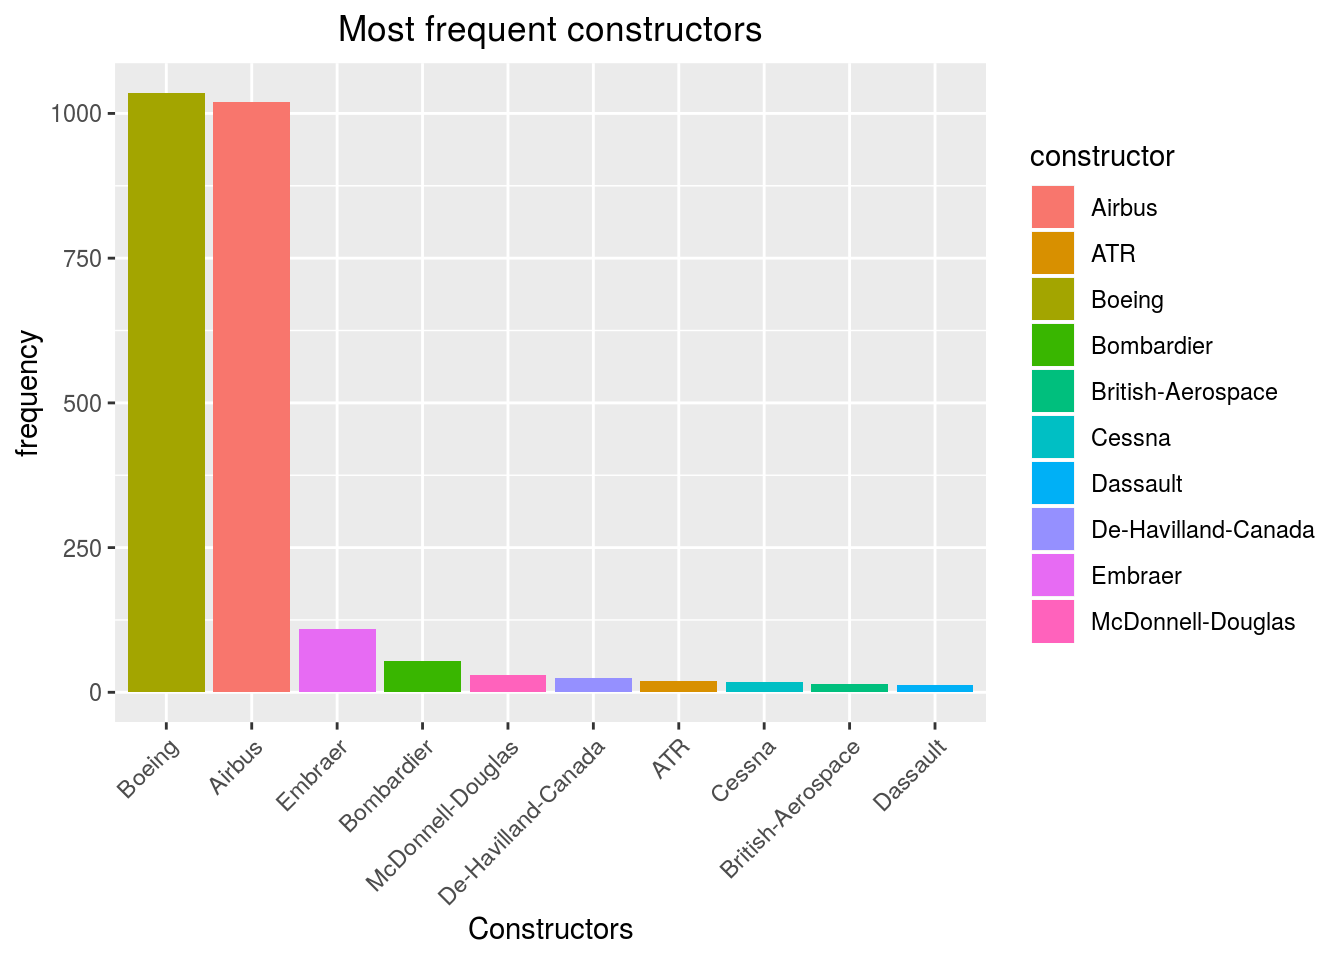
\includegraphics{bookdown-demo_files/figure-latex/unnamed-chunk-9-1} \end{center}

Here we directly anderstand that we won't be able to train a CNN for other constructor than Airbus and Boeing.

\hypertarget{top-airlines}{%
\section{Top airlines}\label{top-airlines}}

\begin{center}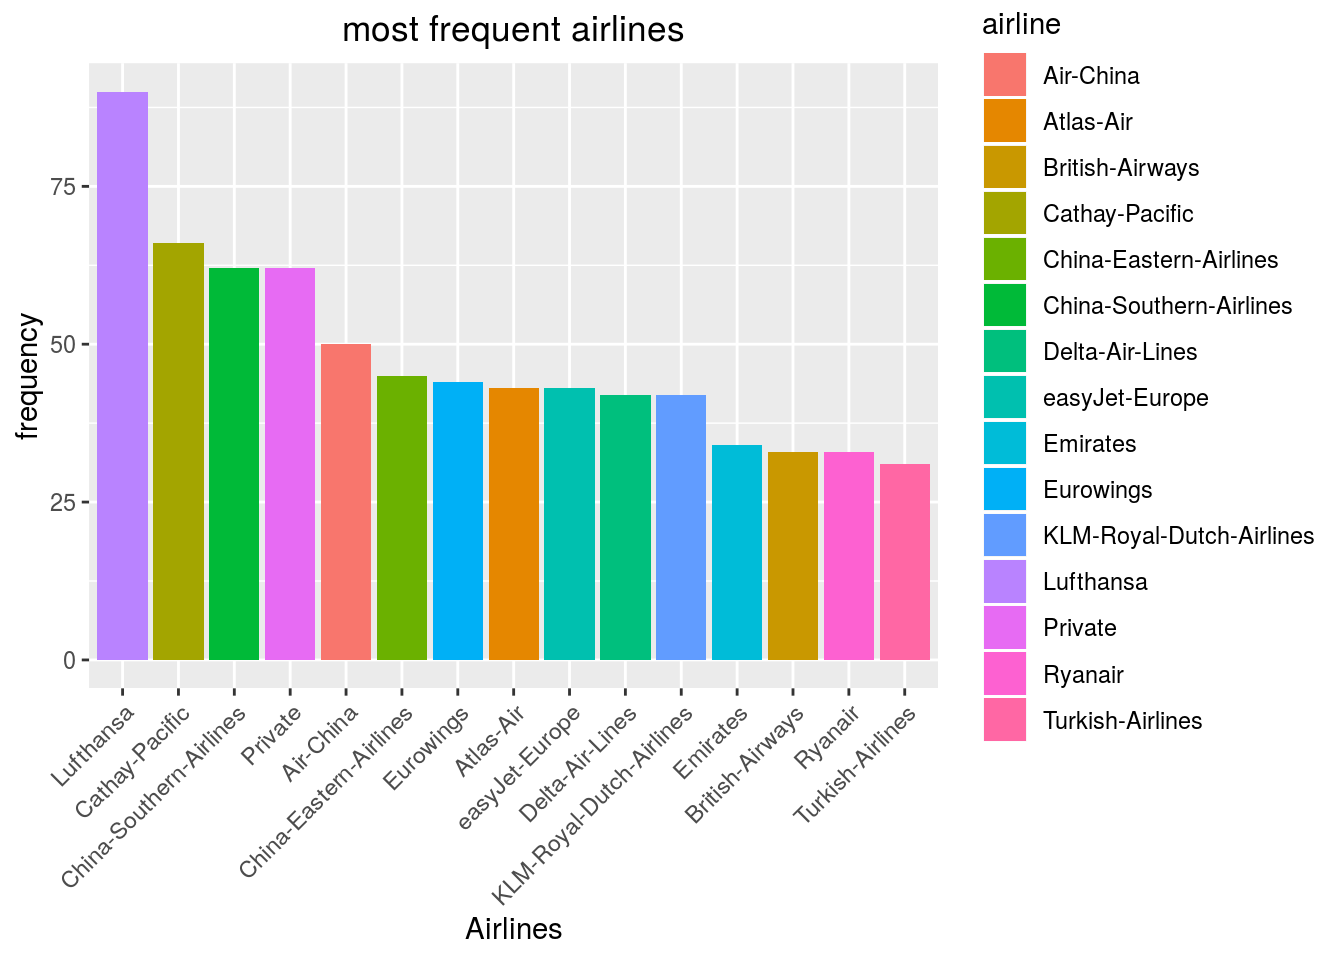
\includegraphics{bookdown-demo_files/figure-latex/unnamed-chunk-11-1} \end{center}

Here, unlike for the constructors the distribution of airlines is more homogeneous, to verify this claim we can plot all of the airlines. So we may be able to train a cnn to recognize the airline of a plane, at least for the most frequent one.

\begin{center}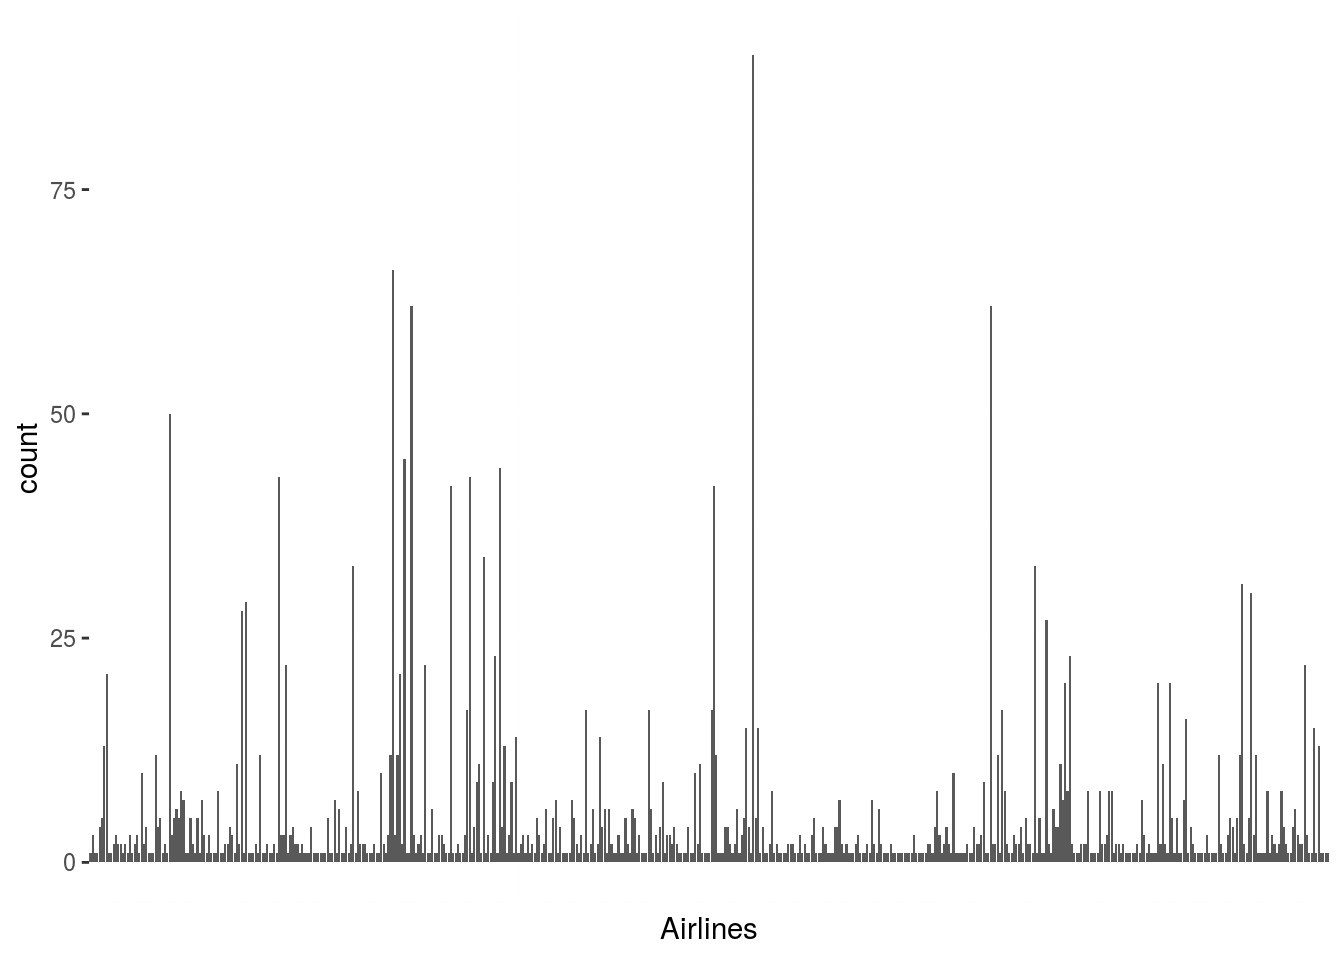
\includegraphics{bookdown-demo_files/figure-latex/unnamed-chunk-12-1} \end{center}

Here we observe there is also a disparity in airlines frequency but much less present than for the constructors.

\hypertarget{proportion-of-model-for-airbus}{%
\section{Proportion of model for Airbus}\label{proportion-of-model-for-airbus}}

\begin{center}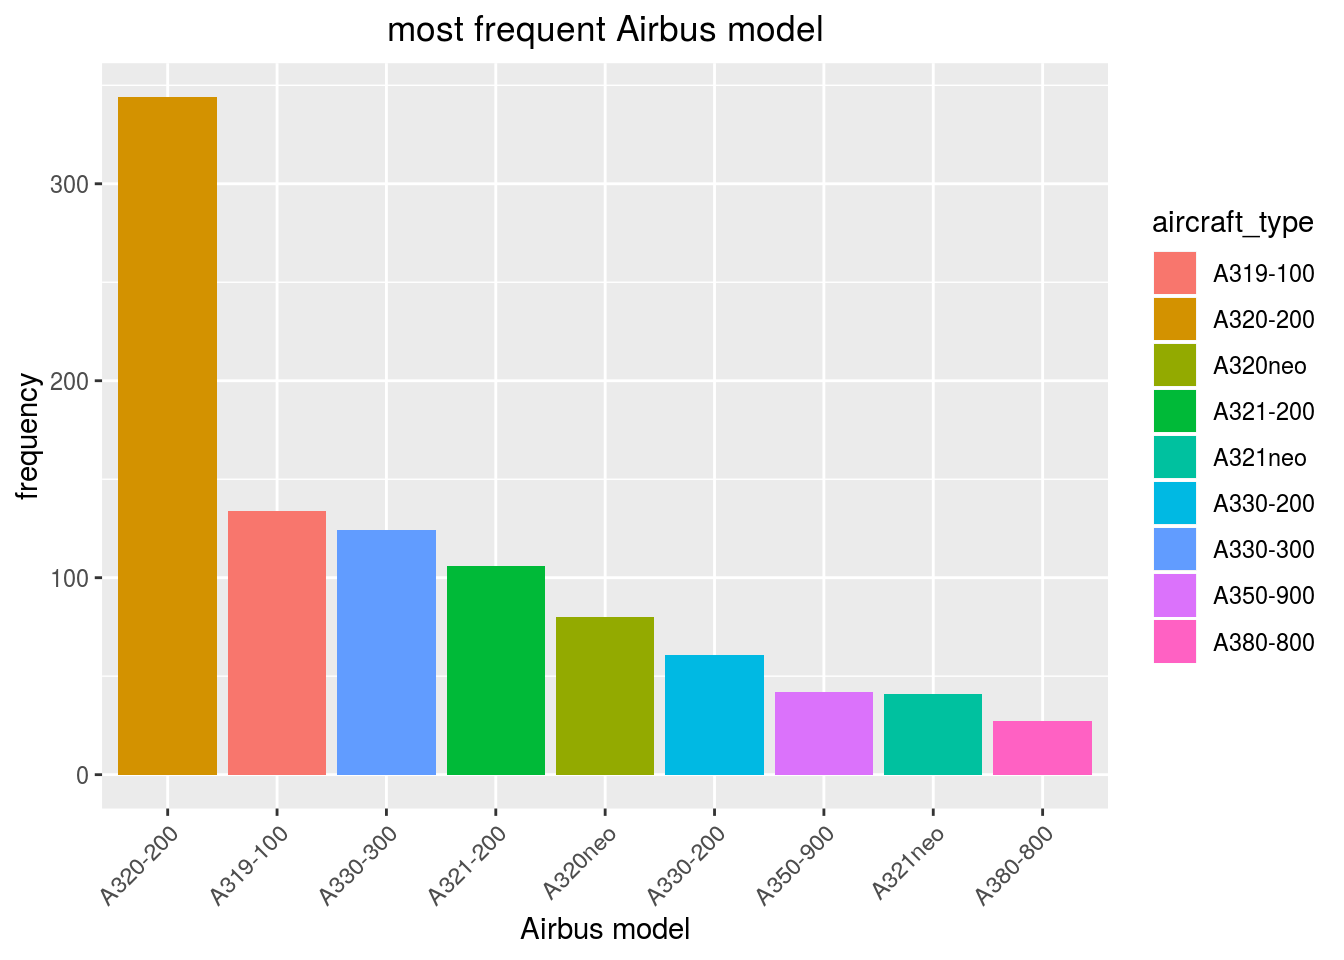
\includegraphics{bookdown-demo_files/figure-latex/unnamed-chunk-14-1} \end{center}

There exist 20 different models of Airbus in our data.
The most frequent Airbus is by far the A320-200.

\hypertarget{proportion-of-model-for-boeing}{%
\section{Proportion of model for Boeing}\label{proportion-of-model-for-boeing}}

\begin{center}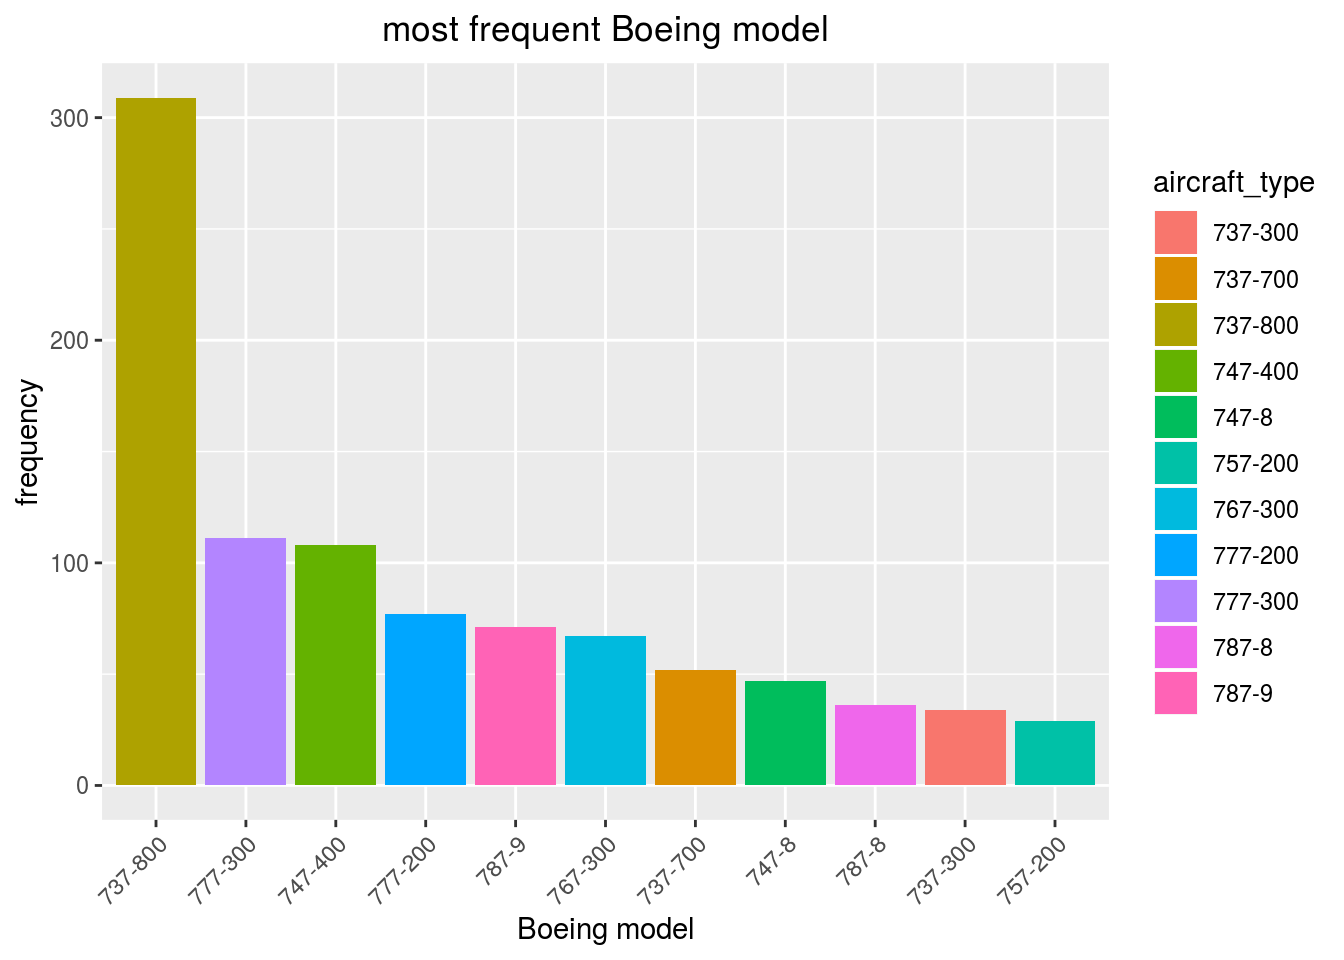
\includegraphics{bookdown-demo_files/figure-latex/unnamed-chunk-16-1} \end{center}

There exist 30 different models of Boeing in our data.
The most frequent Airbus is by far the A320-200.

\hypertarget{deep-learning}{%
\chapter{Deep Learning}\label{deep-learning}}

\hypertarget{overview}{%
\section{Overview}\label{overview}}

The fundamental idea which led to the development of CNN, is the idea that detecting an item in an image should trigger a response (neuron activation) without care for the position in the image of the item. Convolutions ,with filters invariant by translation across the image, follow this idea (\citet{Mallat_2016}).\\
By using several convolutions in parallel and in succession, a network is able to learn some features of the data.
Classification is finally achieved by vectorizing the last layer which feeds a classical multilayer perceptron (MLP).

The first groundbreaking model is \textbf{AlexNet}, developed at the University of Toronto (\citet{NIPS2012_4824}).
It achieved first place at ImageNet image classification competition in 2012.

\begin{figure}
\centering
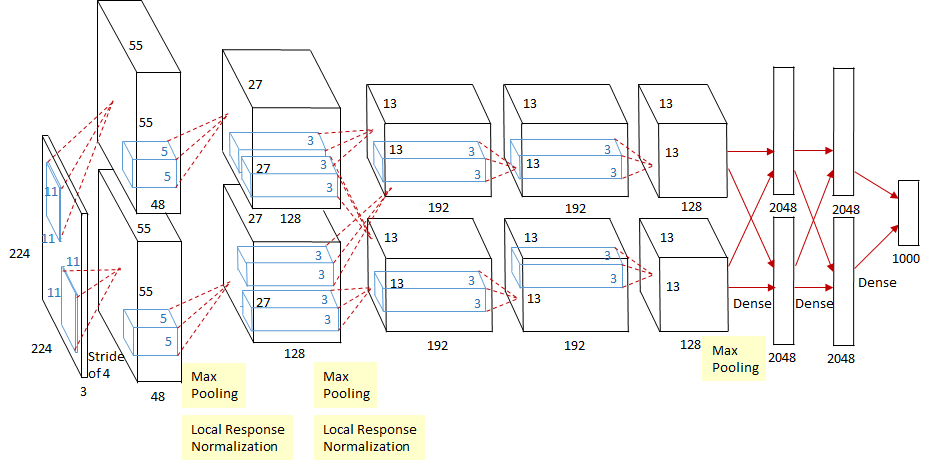
\includegraphics{AlexNetArch.png}
\caption{AlexNet}
\end{figure}

It has many of the features still used today in popular applications.
Several techniques to achieve better results are widespread today :

\begin{itemize}
\tightlist
\item
  ReLU (Rectified Linear Unit) activation : \(ReLU(x) = max(0,x)\)
\item
  Dropout of neurons : some neurons are arbritrarly deactivated
\item
  ensembling several networks
\item
  Data Augmentation : rotations, zooms of images
\item
  Multiple GPUs computation of the backpropagation algorithm (\citet{Rumelhart:1986we}) .
\end{itemize}

For smaller projects, reusing already trained version of popular models on large datasets is also widespread, a technique named `pretraining'.
It usually consists in keeping the convolution layers.

\hypertarget{model}{%
\section{Model}\label{model}}

After several iterations, we have arrived at a model that uses some advanced techniques.
We use Keras (\citet{R-keras}) to implement it.
First, we load a pretrained version on ImageNet dataset of \textbf{VGG16, a CNN developed at Oxford} (\citet{simonyan2014deep}) .
It uses ReLU activation, as seen in AlexNet.
It also uses small, 3 by 3 convolution filters (also named receptive fields), which have been widely adopted in recent years.
In comparison, AlexNet uses 11 by 11 receptive fields.
The training is based on logarithmic loss:
\[H_{y'} (y) := - \sum_{i} y_{i}' \log (y_i)\]
\(y_i\) is the predicted probability value for class \(i\) and \(y_i'\) is the true probability for that class.
Then regularised by L2 weight decay :
\[\mbox{Loss}(w,x) = \mbox{RawLoss}(w,x) + \frac{1}{2} \,\, c \,\|w\|^2\]
On each optimization step in addition to stepping based on a gradient to better fit the training data, all model weights also decay proportionally towards zero by a small factor of \((1-\alpha c)\) , with \(\alpha\) denoting the learning rate (gradient step).
The learning rate is also lowered as time passes, and filters are not initialized randomly.
Dropout (ratio of \(0.5\)) is used in fully-connected layers.
VGG16 structure is as follow.

\begin{verbatim}
## Model
## Model: "vgg16"
## ________________________________________________________________________________
## Layer (type)                        Output Shape                    Param #     
## ================================================================================
## input_2 (InputLayer)                [(None, 150, 150, 3)]           0           
## ________________________________________________________________________________
## block1_conv1 (Conv2D)               (None, 150, 150, 64)            1792        
## ________________________________________________________________________________
## block1_conv2 (Conv2D)               (None, 150, 150, 64)            36928       
## ________________________________________________________________________________
## block1_pool (MaxPooling2D)          (None, 75, 75, 64)              0           
## ________________________________________________________________________________
## block2_conv1 (Conv2D)               (None, 75, 75, 128)             73856       
## ________________________________________________________________________________
## block2_conv2 (Conv2D)               (None, 75, 75, 128)             147584      
## ________________________________________________________________________________
## block2_pool (MaxPooling2D)          (None, 37, 37, 128)             0           
## ________________________________________________________________________________
## block3_conv1 (Conv2D)               (None, 37, 37, 256)             295168      
## ________________________________________________________________________________
## block3_conv2 (Conv2D)               (None, 37, 37, 256)             590080      
## ________________________________________________________________________________
## block3_conv3 (Conv2D)               (None, 37, 37, 256)             590080      
## ________________________________________________________________________________
## block3_pool (MaxPooling2D)          (None, 18, 18, 256)             0           
## ________________________________________________________________________________
## block4_conv1 (Conv2D)               (None, 18, 18, 512)             1180160     
## ________________________________________________________________________________
## block4_conv2 (Conv2D)               (None, 18, 18, 512)             2359808     
## ________________________________________________________________________________
## block4_conv3 (Conv2D)               (None, 18, 18, 512)             2359808     
## ________________________________________________________________________________
## block4_pool (MaxPooling2D)          (None, 9, 9, 512)               0           
## ________________________________________________________________________________
## block5_conv1 (Conv2D)               (None, 9, 9, 512)               2359808     
## ________________________________________________________________________________
## block5_conv2 (Conv2D)               (None, 9, 9, 512)               2359808     
## ________________________________________________________________________________
## block5_conv3 (Conv2D)               (None, 9, 9, 512)               2359808     
## ________________________________________________________________________________
## block5_pool (MaxPooling2D)          (None, 4, 4, 512)               0           
## ================================================================================
## Total params: 14,714,688
## Trainable params: 14,714,688
## Non-trainable params: 0
## ________________________________________________________________________________
\end{verbatim}

We keep the convolution/pooling layers, already trained, and replace the fully connected layer with our own.
The last layer has a sigmoid activation to predict the constructor, either of Airbus or Boeing.

\begin{verbatim}
## Model
## Model: "sequential_1"
## ________________________________________________________________________________
## Layer (type)                        Output Shape                    Param #     
## ================================================================================
## vgg16 (Model)                       (None, 4, 4, 512)               14714688    
## ________________________________________________________________________________
## flatten_1 (Flatten)                 (None, 8192)                    0           
## ________________________________________________________________________________
## dense_2 (Dense)                     (None, 256)                     2097408     
## ________________________________________________________________________________
## dense_3 (Dense)                     (None, 1)                       257         
## ================================================================================
## Total params: 16,812,353
## Trainable params: 16,812,353
## Non-trainable params: 0
## ________________________________________________________________________________
\end{verbatim}

Then, we unfreeze previously frozen layers. This means that some convolution/pooling layers (those after ``block3\_conv1'') are going to be trained even though its
original use was to bring its already trained architecture.
This has shown to boost performance.

\begin{verbatim}
## Model
## Model: "sequential_1"
## ________________________________________________________________________________
## Layer (type)                        Output Shape                    Param #     
## ================================================================================
## vgg16 (Model)                       (None, 4, 4, 512)               14714688    
## ________________________________________________________________________________
## flatten_1 (Flatten)                 (None, 8192)                    0           
## ________________________________________________________________________________
## dense_2 (Dense)                     (None, 256)                     2097408     
## ________________________________________________________________________________
## dense_3 (Dense)                     (None, 1)                       257         
## ================================================================================
## Total params: 16,812,353
## Trainable params: 16,552,193
## Non-trainable params: 260,160
## ________________________________________________________________________________
\end{verbatim}

We perform some data augmentation: rotation, zoom, horizontal flip.

\begin{Shaded}
\begin{Highlighting}[]
\NormalTok{train_datagen =}\StringTok{ }\KeywordTok{image_data_generator}\NormalTok{(}
  \DataTypeTok{rescale =} \DecValTok{1}\OperatorTok{/}\DecValTok{255}\NormalTok{,}
  \DataTypeTok{rotation_range =} \DecValTok{40}\NormalTok{,}
  \DataTypeTok{width_shift_range =} \FloatTok{0.2}\NormalTok{,}
  \DataTypeTok{height_shift_range =} \FloatTok{0.2}\NormalTok{,}
  \DataTypeTok{shear_range =} \FloatTok{0.2}\NormalTok{,}
  \DataTypeTok{zoom_range =} \FloatTok{0.2}\NormalTok{,}
  \DataTypeTok{horizontal_flip =} \OtherTok{TRUE}\NormalTok{,}
  \DataTypeTok{fill_mode =} \StringTok{"nearest"}
\NormalTok{)}
\end{Highlighting}
\end{Shaded}

Skipping some technical details, we arrive at the training step. Here we use binary crossentropy (aka logarithmic loss) as a loss function.
Moreover, we store classification accuracy, the ratio of number of correct predictions to the total number of images classified.

\[Acc = \frac{TP + TN}{TP+TN+FP+FN}\]
where: TP = True positive; FP = False positive; TN = True negative; FN = False negative.

\begin{Shaded}
\begin{Highlighting}[]
\NormalTok{model }\OperatorTok\StringTok{ }\KeywordTok{compile}\NormalTok{(}
  \DataTypeTok{loss =} \StringTok{"binary_crossentropy"}\NormalTok{,}
  \DataTypeTok{optimizer =} \KeywordTok{optimizer_rmsprop}\NormalTok{(}\DataTypeTok{lr =} \FloatTok{1e-5}\NormalTok{),}
  \DataTypeTok{metrics =} \KeywordTok{c}\NormalTok{(}\StringTok{"accuracy"}\NormalTok{)}
\NormalTok{)}
\end{Highlighting}
\end{Shaded}

Then we can train the model.
Here we used 100 epochs with 100 steps by epoch.

\begin{Shaded}
\begin{Highlighting}[]
\NormalTok{history <-}\StringTok{ }\NormalTok{model }\OperatorTok\StringTok{ }\KeywordTok{fit_generator}\NormalTok{(}
\NormalTok{  train_generator,}
  \DataTypeTok{steps_per_epoch =} \DecValTok{100}\NormalTok{,}
  \DataTypeTok{epochs =} \DecValTok{100}\NormalTok{,}
  \DataTypeTok{validation_data =}\NormalTok{ validation_generator,}
  \DataTypeTok{validation_steps =} \DecValTok{50}
\NormalTok{)}
\end{Highlighting}
\end{Shaded}

\hypertarget{performance-check}{%
\section{Performance check}\label{performance-check}}

We iterated over several models.
In the following images, we plot the logarithmic loss and the accuracy, on both the training and validation data for each of them.
First, we implemented our own convolution layers and fully connected layers.
In this model, we only use 30 epochs since we do not augment the dataset. Our loss reaches a minimum at around 15 epochs on the validation set.
The validation accuracy begins to decrease after 25 epochs.
The model achieves around 80\% accuracy.

\begin{figure}
\centering
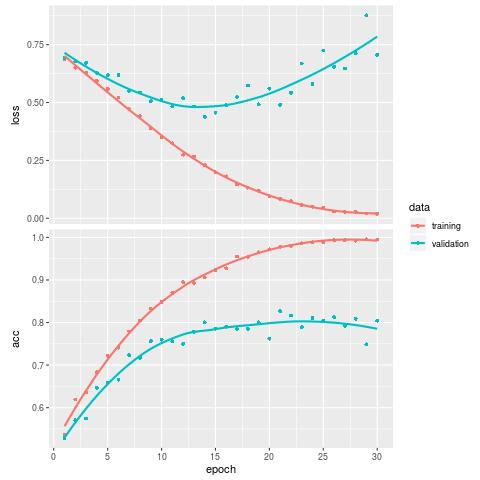
\includegraphics{history-CNN-scratch_full.jpg}
\caption{Introductory model}
\end{figure}

\clearpage

After this first iteration, we then performed image augmentation, which allow us to use 100 epochs.
The validation loss reaches a minimum at around 80 epochs.
However, accuracy on the validation set decreased to 70\%.

\begin{figure}
\centering
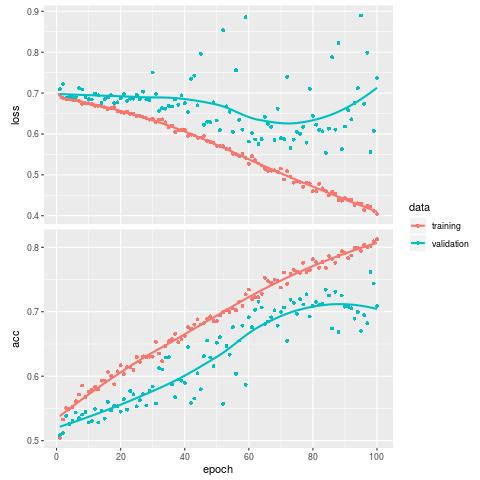
\includegraphics{history-CNN-augmented-scratch.jpg}
\caption{Model with augmented images}
\end{figure}

\clearpage

At this point, we considered adding pretrained convolution layers from VGG16.
We only train the fully connected layers, thus we use 30 epochs.
Here, the validation and train loss are curiously intertwined.
The accuracy does not reach a plateau, and is of 70\% at the last epoch.

\begin{figure}
\centering
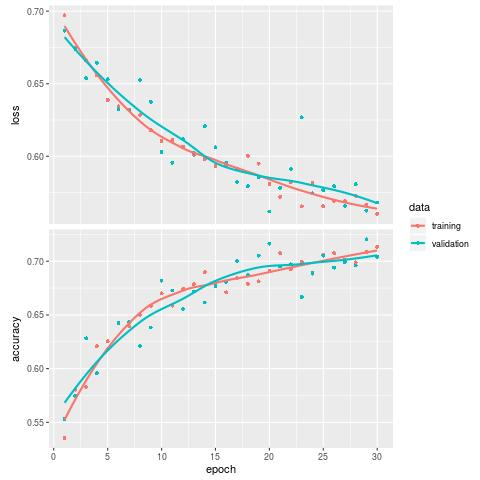
\includegraphics{history-CNN-augmented-pretrained.jpg}
\caption{Model with pretraining}
\end{figure}

\clearpage

Lastly, we unfroze part of VGG16 convolution layers.
This is the model discussed in the previous part.
We resort to 100 epochs and observe a more classical loss, with the validation loss going up after 30 epochs while the training one continues downwards.
The validation accuracy finally reaches 88\%, plateauing at 30 epochs with 85\% but still slowing growing afterwards.

\begin{figure}
\centering
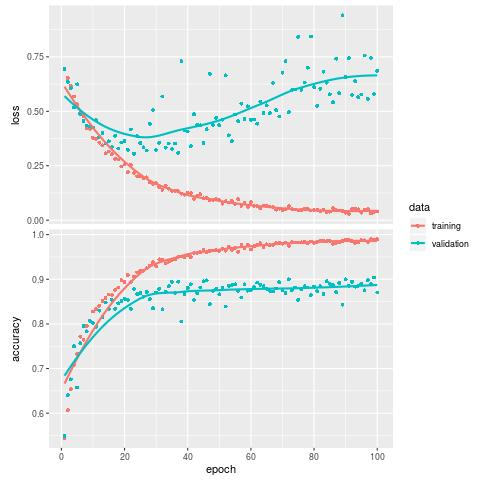
\includegraphics{history-CNN-augmented-pretrained-fine-tunning.jpg}
\caption{Final model}
\end{figure}

\clearpage

\hypertarget{putting-into-production}{%
\chapter{Putting into production}\label{putting-into-production}}

\hypertarget{rest-api-with-plumber}{%
\section{REST API with Plumber}\label{rest-api-with-plumber}}

Technically, API stands for Application Program Interface --- a name that's both exactly what an API is and too vague to actually convey any meaning. But what are API's really? They're a simple way to set up a computer to pass information to other computers through the internet. 95\% of the time, when people say API they mean a RESTful API, which is an API that uses HTTP to interact with other computers. HTTP is the same protocol your browser is using for you to read websites. When you type in a URL to a website, a computer receives your request and sends back HTML. RESTful API's are the same thing, but instead of HTML they send back text or data.

When you call an API you typically do one of two things. You either request that computer to send you a specific piece of information (like the weather of a certain city you requested), or you ask the other computer to change the data it has stored (like adding a record to a table). Most simply, API's are ways to --- from your computer --- call a function on another computer.

The easiest way to create an API in R is using the library plumber (\citet{R-plumber}), a package which can convert existing R code into an API with just a few extra lines.

First, we create a script that loads the data and trains the model.

\textbf{runtime\_functions.R}

\begin{Shaded}
\begin{Highlighting}[]
\KeywordTok{library}\NormalTok{(keras)}

\NormalTok{model <-}\StringTok{ }\KeywordTok{load_model_hdf5}\NormalTok{(}\StringTok{"plane-spotter_pretrained_fine_tuning.h5"}\NormalTok{)}

\NormalTok{image_prediction <-}\StringTok{ }\ControlFlowTok{function}\NormalTok{(path)\{}
\NormalTok{  image <-}\StringTok{ }\KeywordTok{image_load}\NormalTok{(path, }\DataTypeTok{target_size =} \KeywordTok{c}\NormalTok{(}\DecValTok{150}\NormalTok{,}\DecValTok{150}\NormalTok{)) }\OperatorTok\StringTok{ }
\StringTok{    }\KeywordTok{image_to_array}\NormalTok{() }\OperatorTok\StringTok{ }
\StringTok{    }\KeywordTok{array_reshape}\NormalTok{(}\KeywordTok{c}\NormalTok{(}\DecValTok{1}\NormalTok{, }\DecValTok{150}\NormalTok{, }\DecValTok{150}\NormalTok{, }\DecValTok{3}\NormalTok{))}
\NormalTok{  image_tensor <-}\StringTok{ }\NormalTok{image}\OperatorTok{/}\DecValTok{255}
\NormalTok{  pred <-}\StringTok{ }\KeywordTok{predict_classes}\NormalTok{(model, image_tensor)}
  \ControlFlowTok{if}\NormalTok{(pred }\OperatorTok{==}\StringTok{ }\DecValTok{0}\NormalTok{)\{}
    \KeywordTok{return}\NormalTok{(}\StringTok{"Airbus"}\NormalTok{)}
\NormalTok{  \} }\ControlFlowTok{else}\NormalTok{\{}
    \KeywordTok{return}\NormalTok{(}\StringTok{"Boeing"}\NormalTok{)}
\NormalTok{  \}}
\NormalTok{\}}

\KeywordTok{image_prediction}\NormalTok{(}\StringTok{"Plumber/Boeing.5023.jpg"}\NormalTok{)}
\end{Highlighting}
\end{Shaded}

The output is ``Boeing''

Then we built the GET endpoint :

\textbf{rest\_controller.R}

\begin{Shaded}
\begin{Highlighting}[]
\KeywordTok{source}\NormalTok{(}\StringTok{"runtime_functions.R"}\NormalTok{)}

\CommentTok{# Set an endpoint to return a pet name}
\CommentTok{#* @get /names}
\NormalTok{get_names <-}\StringTok{ }\ControlFlowTok{function}\NormalTok{()\{}
  \KeywordTok{image_prediction}\NormalTok{(}\StringTok{"Plumber/Boeing.5023.jpg"}\NormalTok{)}
\NormalTok{\}}
\end{Highlighting}
\end{Shaded}

Here for the purpose of the exemple we predict a known image but the aim of the API is to get the image path as the input of the function.

Finally, we need to use plumber to set up our R code to accept HTTP requests and transform them into executable R code.

We simply:

\begin{enumerate}
\def\labelenumi{\arabic{enumi}.}
\tightlist
\item
  Import plumber.
\item
  Show plumber where our endpoints are.
\item
  Start the API service on port 80.
  Since HTTP defaults to port 80, our service to that port allows things we type in our browser to be executed in the R on our computer.
\end{enumerate}

\textbf{Main.R}

\begin{Shaded}
\begin{Highlighting}[]
\KeywordTok{library}\NormalTok{(plumber)}

\NormalTok{r <-}\StringTok{ }\KeywordTok{plumb}\NormalTok{(}\StringTok{"rest_controller.R"}\NormalTok{)}
\NormalTok{r}\OperatorTok{$}\KeywordTok{run}\NormalTok{(}\DataTypeTok{port=}\DecValTok{80}\NormalTok{, }\DataTypeTok{host=}\StringTok{"0.0.0.0"}\NormalTok{)}
\end{Highlighting}
\end{Shaded}

Great, now we can see the result of the output either by typing curl -X GET ``\url{http://127.0.0.1:6974/names}'' -H ``accept: application / json'' on the terminal or directly by going to \url{http://127.0.0.1:6974/names} in your browser.

\hypertarget{docker}{%
\section{Docker}\label{docker}}

As a data scientist, we sometimes want to have code running in places that are not our computer. In our case, we want to have our R script run an API continuously, regardless of if our laptop runs out of battery.
One way we could set this up would be to create a virtual machine in a place like Amazon Web Services. A virtual machine is like a computer that you've used before, but it's simulated--it doesn't have it's own process, memory, or hardware. Instead, a different computer is running the machine. Virtual machines are great because many of them can run on a single server, and they can be easily started and stopped.

Docker is a way to make the process of configuring and running computers smoother. With Docker, you can create a single document that specifies how to set up the computer. The document lets you run these steps at a moments notice. More formally, docker is a way to run virtual machines as containers, which are lightweight executable packages of software. A container is an instance of an image, which is a snapshot of a computer at a moment in time. Images can be full snapshots, or they can just be a small addition to an earlier image. A dockerfile is the specification document for how to build the image.

So we try to use the API we created as the code we want in our docker container. We'll start with an image already setup to have Linux on it. Then we'll create an image that has R installed on top of Linux. After that, we'll add our R libraries into a third image. Lastly, we'll transfer our files to the final image.

A great thing about Docker is that since so many people use it, you can often find images that other people have made that do what you want to do. In our case, the Rocker project has a ton of Docker images that support R.
In order to build an image, Docker always looks for a plain text file with no extension called dockerfile.

To customize our docker container, we first specify our base container. For us, that's the rocker/r-ver:3.5.0 image. We do this by using the \texttt{FROM} command. Then, we need to install the linux packages that are required for the plumber using linux bash commands. To these commands while setting up the image, we use the \texttt{RUN}. We then install python and the different usefull libraries, and \texttt{COPY} our code in the container.

And that's our dockerfile! It builds everything we need to run our API from any machine, regardless of the setup! All together it looks like this:

\begin{verbatim}
FROM rocker/r-ver:3.6.0

# update some packages, including sodium and apache2, then clean
RUN apt-get update \
  && apt-get install -y --no-install-recommends \
    file \
    libcurl4-openssl-dev \
    libedit2 \
    libssl-dev \
    lsb-release \
    psmisc \
    procps \
    wget \
    libxml2-dev \
    libpq-dev \
    libssh2-1-dev \
    ca-certificates \
    libglib2.0-0 \
    libxext6 \
    libsm6  \
    libxrender1 \
    bzip2 \
    libsodium-dev \
    apache2 \
    zlib1g-dev \
    && wget -O libssl1.0.0.deb http://ftp.debian.org/debian/pool/main/o/openssl/libssl1.0.0_1.0.1t-1+deb8u8_amd64.deb \
    && dpkg -i libssl1.0.0.deb \
    && rm libssl1.0.0.deb \
    && apt-get clean \
    && rm -rf /var/lib/apt/lists/

# install miniconda, and set the appropriate path variables.
RUN wget --quiet https://repo.anaconda.com/miniconda/Miniconda3-4.6.14-Linux-x86_64.sh -O ~/miniconda.sh && \
    /bin/bash ~/miniconda.sh -b -p /opt/conda && \
    rm ~/miniconda.sh && \
    /opt/conda/bin/conda clean -tipsy && \
    ln -s /opt/conda/etc/profile.d/conda.sh /etc/profile.d/conda.sh && \
    echo ". /opt/conda/etc/profile.d/conda.sh" >> ~/.bashrc && \
    echo "conda activate base" >> ~/.bashrc
ENV PATH /opt/conda/bin:$PATH

# install tensorflow and h5py using the pip that links to miniconda (the default pip is for python 2.7)
RUN /opt/conda/bin/pip install --no-cache-dir tensorflow==2.0.0 h5py==2.10.0

# install Pillow to load a unique image
RUN /opt/conda/bin/pip install PIL
RUN /opt/conda/bin/pip install Pillow


# let R know the right version of python to use
ENV RETICULATE_PYTHON /opt/conda/bin/python

# copy the setup script, run it, then delete it
COPY src/setup.R /
RUN Rscript setup.R && rm setup.R

# copy all the other R files.
COPY src /src

EXPOSE 80

WORKDIR /src
ENTRYPOINT ["Rscript","main.R"]
\end{verbatim}

To build our image, open a terminal in the project folder and run
`\texttt{docker\ build\ -t\ r-tensorflow-api\ .}

And in order to run the container :
\texttt{docker\ run\ -\/-rm\ -it\ -p\ 80:80\ r-tensorflow-api}

If you want to have this web service running on a server in the cloud, it only takes a few more steps. One way to do this is to use a tool like Amazon Elastic Container Service (ECS). ECS lets you take a container you've created and deploy it to AWS. At that point your container is running within AWS systems, and you will get an endpoint that anyone can hit with a browser from anywhere.

\hypertarget{conclusion}{%
\chapter{Conclusion}\label{conclusion}}

Our final model achieves around 88\% accuracy, on validation images, at binary classification of Airbus versus Boeing airplanes.

The next step would be to classify model types.
To do so, we could chain another CNN:

\begin{enumerate}
\def\labelenumi{\arabic{enumi}.}
\tightlist
\item
  an image is classified under Airbus or Boeing by our binary CNN.
\item
  the image is then fed into either one of two models trained to recognize model types of Boeing or Airbus, respectively.
\end{enumerate}

(e.g.~if our first model outputs our image as Airbus, we feed the image in the Airbus model type CNN)
The output is the model of the airplane. To achieve this, we need to scrape the website again.
Sadly, the website \href{https://www.planespotters.net/}{\textbf{planespotters.net}} was totally redesigned which made our scrapping code obsolete.

In the end, we achieved a reasonable objective to scrap a website to obtain data, explore the data, train a deep learning model, create an API and a docker image.
We also obtained a CNN able to differenciate Airbus and Boeing airplaines.
Further advance would require rebuilding a scrapping tool.
Moreover, our dataset size of around two thousand images (not counting augmentation), is a bit limited.

In the computer vision community, several other methods are being developed which grow in popularity (\citet{DBLP:journals/corr/GuWKMSSLWW15}).
For example, stochastic gradient descent (or its relaxation to a few samples, minibatch) associated with batch normalization seem promising.
Inception modules also allow to reduce the number of parameters (reduced to 5 millions which are much less than AlexNet with 60 millions).
Residual Nets (ResNets) are also growing in popularity.

\bibliography{biblio.bib,packages.bib}

\end{document}
